\documentclass[tikz,convert={outfile=\jobname.svg}]{standalone}
\usepackage[utf8]{inputenc}
\usepackage[TS1,OT1]{fontenc}% or T1 instead of OT1
\newcommand{\longs}{{\fontencoding{TS1}\fontfamily{lmr}\selectfont\char115}} 
\usetikzlibrary{calc}
\usetikzlibrary{decorations.pathreplacing}
\usetikzlibrary{shapes}
\begin{document}
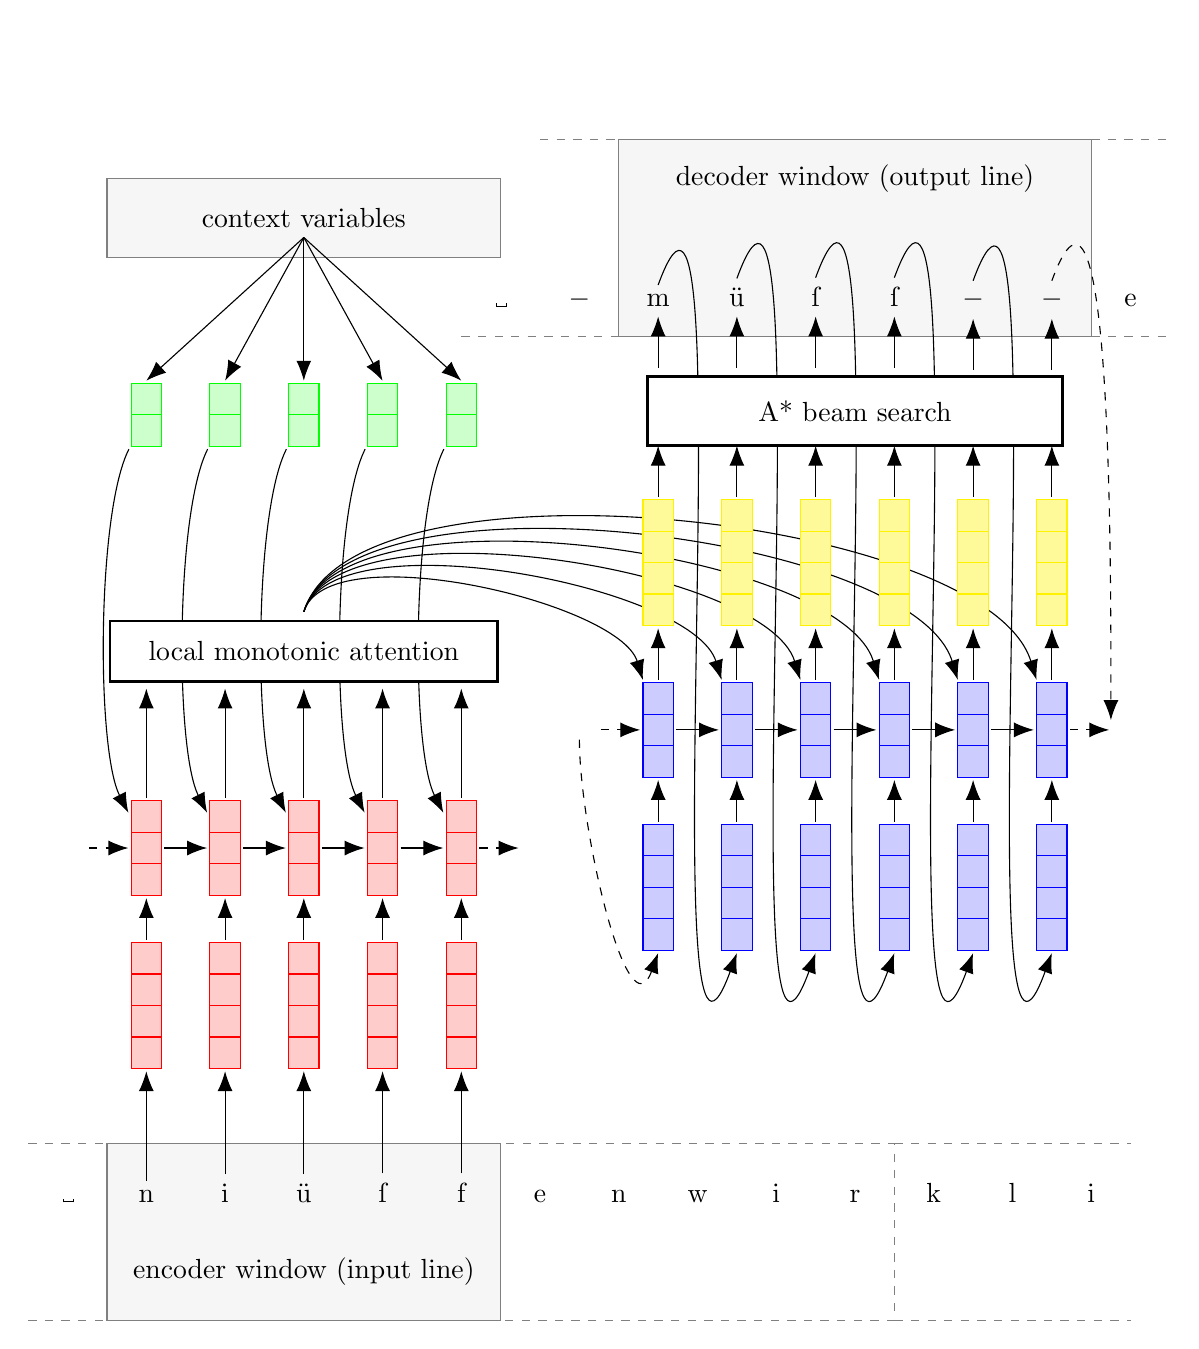
\begin{tikzpicture}[
  scale=0.5,
  hid/.style 2 args={
    rectangle split,
    rectangle split,
    draw=#2,
    rectangle split parts=#1,
    fill=#2!20,
    outer sep=1}]
  \usetikzlibrary{calc,arrows.meta}
  \pgfdeclarelayer{background}
  \pgfdeclarelayer{foreground}
  \pgfsetlayers{background,main,foreground}
  % show context variables rectangle
  \draw[gray,fill=gray!10,fill opacity=0.7,text opacity=1] (-1,14) rectangle (9,16);
  \node (context) at (4, 15) {context variables};
  % draw context embedding nodes
  \foreach \step in {1,...,5} {
    \node[hid={2}{green}] (c\step) at (2*\step-2, 10) {};
    \draw[-{Latex[scale=1.5]}] (context.south) -> (c\step.north);
  }
  % show input window rectangle
  \draw[gray,dashed] (-3,-13) -- (-1,-13);
  \draw[gray,dashed] (-3,-8.5) -- (-1,-8.5);
  \draw[gray,fill=gray!10,fill opacity=0.7,text opacity=1] (-1,-13) rectangle (9,-8.5);
  \draw[gray,dashed] (9,-13) rectangle (19,-8.5);
  \draw[gray,dashed] (19,-13) -- (25,-13);
  \draw[gray,dashed] (19,-8.5) -- (25,-8.5);
  \node (iwindow) at (4, -11.75) {encoder window (input line)};
  % draw input nodes
  \foreach \i [count=\step from 0] in {\textvisiblespace,n,i,ü,\longs,f,e,n,w,i,r,k,l,i}
    \node[align=center,anchor=base] (i\step) at (2*\step-2, -10) {\rmfamily\i};
  % show output window rectangles
  \draw[gray,dashed] (8,12) -- (12,12);
  \draw[gray,dashed] (10,17) -- (12,17);
  \draw[gray,fill=gray!10,fill opacity=0.7,text opacity=1] (12,12) rectangle (24,17);
  \draw[gray,dashed] (24,12) -- (26,12);
  \draw[gray,dashed] (24,17) -- (26,17);
  \node (owindow) at (18, 16) {decoder window (output line)};
  % draw output nodes
  \newcommand{\gapsymbol}{$-$} %$\varepsilon$, $\emptyset$ $\varnothing$
  \foreach \t [count=\step from 4] in {\textvisiblespace,\gapsymbol,m,ü,\longs,\longs,\gapsymbol,\gapsymbol,e} {
    \node[align=center,anchor=base] (o\step) at (2*\step+1, +12.75) {\rmfamily\t};
  }
  % draw embedding and hidden layers for encoder
  \foreach \step in {1,...,5} {
    \node[hid={3}{red}] (h\step) at (2*\step-2, -1) {};
    \node[hid={4}{red}] (e\step) at (2*\step-2, -5) {};    
    \node               (a\step) at (2*\step-2, 3.3) {};    
    \draw[-{Latex[scale=1.5]}] (i\step.north) -> (e\step.south);
    \draw[-{Latex[scale=1.5]}] (e\step.north) -> (h\step.south);
    \draw[-{Latex[scale=1.5]}] (h\step.north) -> (a\step.south);
    \path (c\step) edge[-{Latex[scale=1.5]},out=243,in=117,looseness=0.5] (h\step);
  }
  % draw embedding and hidden layers for decoder
  \foreach \step in {6,...,11} {
    \node[hid={4}{yellow},fill=yellow!40] (s\step) at (2*\step+1, 6.25) {};
    \node[hid={3}{blue}] (h\step) at (2*\step+1, 2) {};
    \node[hid={4}{blue}] (e\step) at (2*\step+1, -2) {};    
    \draw[-{Latex[scale=1.5]}] (e\step.north) -> (h\step.south);
    \draw[-{Latex[scale=1.5]}] (h\step.north) -> (s\step.south);
    \draw[-{Latex[scale=1.5]}] (s\step.north) -> +(up:1.3);
    \draw[-{Latex[scale=1.5]}] (o\step.south)+(down:1.3) -> (o\step.south);
  }  
  % draw recurrent links
  \foreach \step in {1,...,4} {
    \pgfmathtruncatemacro{\next}{add(\step,1)}
    \draw[-{Latex[scale=1.5]}] (h\step.east) -> (h\next.west);
  }
  \draw[-{Latex[scale=1.5]},dashed] (h5.east) -> +(right:1);
  \draw[-{Latex[scale=1.5]},dashed] (h1.west)+(left:1) -> (h1.west);
  \foreach \step in {6,...,10} {
    \pgfmathtruncatemacro{\next}{add(\step,1)}
    \draw[-{Latex[scale=1.5]}] (h\step.east) -> (h\next.west);
  }
  \draw[-{Latex[scale=1.5]},dashed] (h11.east) -> +(right:1);
  \draw[-{Latex[scale=1.5]},dashed] (h6.west)+(left:1) -> (h6.west);
  % beam search box for LM prediction
  \begin{pgfonlayer}{foreground}
    \node (beamsearch) at (18,10.1) [draw,thick,minimum width=150,minimum height=25,fill=white] {A* beam search};
  \end{pgfonlayer}{foreground}
  % draw predicted-labels-as-inputs links
  \foreach \step in {6,...,10} {
    \pgfmathtruncatemacro{\next}{add(\step,1)}
    \path (o\step.north) edge[-{Latex[scale=1.5]},out=70,in=250] (e\next.south);
  }
  % edge case: draw edge for special input token
  \node (h11post) at (2*11+2.5, 2) {};
  \path (o11.north) edge[-{Latex[scale=1.5]},dashed,out=70,in=90] (h11post);
  \node (h6pre) at (2*6-1, 2) {};
  \path (h6pre) edge[-{Latex[scale=1.5]},dashed,out=270,in=250] (e6.south);
  % attention/peeking box for transfer
  \node (attention) at (4,4) [draw,thick,minimum width=140,minimum height=22,fill=white] {local monotonic attention};
    \begin{pgfonlayer}{background}
    \foreach \step in {6,...,11} {
      \path (4,5) edge[-{Latex[scale=1.5]},out=73,in=107,looseness=0.6] (h\step);
    }
    \end{pgfonlayer}
  \end{tikzpicture}%
\end{document}
